% GET pipeline — keyword-to-stage assignment (SPEC.md §5.5).
% Companion to algorithm-get: the stages in order, with the keywords each
% stage consumes. Stage order is normative.
\documentclass[border=6pt]{standalone}
\usepackage[T1]{fontenc}
\usepackage{tikz}
\usetikzlibrary{positioning,arrows.meta}
\begin{document}
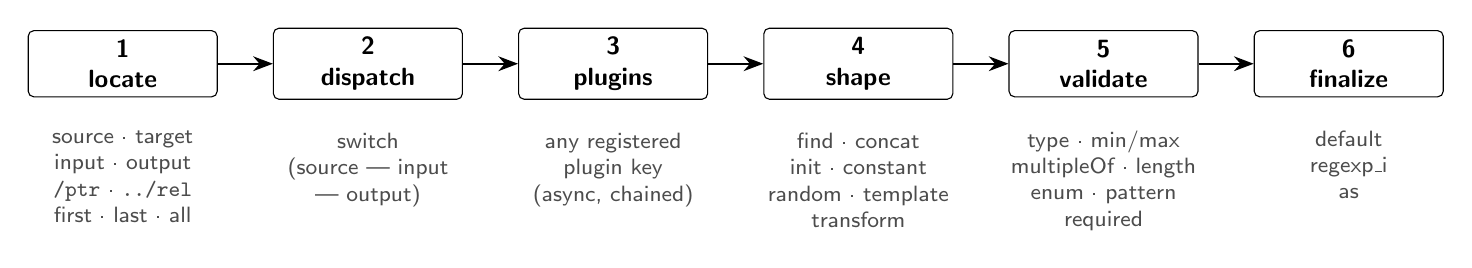
\begin{tikzpicture}[
  font=\sffamily,
  stage/.style={draw, rounded corners=2pt, minimum height=8mm, minimum width=24mm, align=center, font=\sffamily\bfseries\small},
  kw/.style={align=center, font=\sffamily\footnotesize, text=black!70},
  flow/.style={-{Stealth[length=2.5mm]}, thick}
]
  \node[stage] (locate) {1\\locate};
  \node[stage, right=7mm of locate] (dispatch) {2\\dispatch};
  \node[stage, right=7mm of dispatch] (plugins) {3\\plugins};
  \node[stage, right=7mm of plugins] (shape) {4\\shape};
  \node[stage, right=7mm of shape] (validate) {5\\validate};
  \node[stage, right=7mm of validate] (finalize) {6\\finalize};

  \draw[flow] (locate) -- (dispatch);
  \draw[flow] (dispatch) -- (plugins);
  \draw[flow] (plugins) -- (shape);
  \draw[flow] (shape) -- (validate);
  \draw[flow] (validate) -- (finalize);

  \node[kw, below=3mm of locate] {source · target\\input · output\\\texttt{/ptr} · \texttt{../rel}\\first · last · all};
  \node[kw, below=3mm of dispatch] {switch\\(source | input\\| output)};
  \node[kw, below=3mm of plugins] {any registered\\plugin key\\(async, chained)};
  \node[kw, below=3mm of shape] {find · concat\\init · constant\\random · template\\transform};
  \node[kw, below=3mm of validate] {type · min/max\\multipleOf · length\\enum · pattern\\required};
  \node[kw, below=3mm of finalize] {default\\regexp\_i\\as};
\end{tikzpicture}
\end{document}
